\documentclass[a4paper,12pt]{article}
\usepackage{blindtext}
\usepackage[utf8]{inputenc}
\usepackage{graphicx}
\usepackage{enumitem}

\begin{document}
\begin{titlepage}
\center

\textsc{\LARGE Functional Requirements and Application Design}\\[1.5cm]
\textsc{\Large Project: Traffic Camera Image Analysis}\\[1.5cm]
\textsc{\large Client: DPSS, CSIR}\\[0.5cm]
\textsc{\large Team: Quadcore Productions}\\[0.5cm]

\begin{minipage}{0.4\textwidth}
\begin{flushleft} \large
\emph{Author(s):}\\
Mpho \textsc{Baloyi}\\
Hlengekile \textsc{Jita}\\
Mayimela \textsc{Moses}\\
Mbhele \textsc{Themba}\\
\end{flushleft}
\end{minipage}
~
\begin{minipage}{0.4\textwidth}
\begin{flushright} \large
\emph{Student number(s):} \\
14133670\\ % Student number
14077893\\
14019702\\
14007950\\
\end{flushright}
\end{minipage}\\

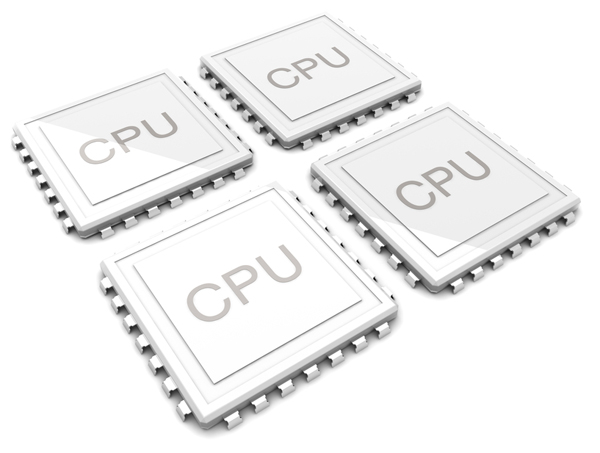
\includegraphics[width=\textwidth]{2012-quad-core-phones.jpg}

{\large University of Pretoria, Department of Computer Science}\\

{\large 27 May 2016}\\[3cm]

\vfil

\end{titlepage}

\newpage
\tableofcontents
\newpage
\section{Introduction}
This document describes the functional requirements and application design of the Traffic Camera Image Analysis System. The target system will run on a web server  and be accessed by users on an Android Application which will provide the users with the necessary functionality to access real-time traffic information that assists them with things such as avoiding traffic and choosing the best alternative routes. 

In this specification, we cover the use cases, their service contracts, required functionality and process specifications of the target system. The above, will be built on over time as the software is developed, as we are following an agile development methodology. In addition the domain model of the application as a whole will be provided.
\section{Vision}
For this project we aim to achieve a system that makes use of images obtained from highway cameras to provide users with up-to-date real-time traffic information. The system should simplify the user's travels by providing traffic information and notifying them before they depart of traffic conditions, calculating arrival times based on traffic conditions and help them select the most suitable route for their trips using the traffic information and additional metrics. Our vision for the target system is that it should be reliable and perform relatively quickly, both for user satisfaction and in order to be the an up-to-date traffic information system.
\section{Background}
As a commuter, traffic is something that is a part of everyday life, and it is not one of the more pleasurable aspects of life. Already there is software in place that assists us in dealing with this problem, such as Google Maps. This software uses the crowd-sourcing of GPS data in order to provide their up-to-date traffic information.

In our system,we want to take an image analysis approach to solve the same problem. We will make use of the publicly available SANRAL highway cameras to get images which can be found on https://www.i-traffic.co.za/traffic/cameras.aspx. Processing these images we will perform image analysis and determine the traffic conditions in the area of a camera. Using this information we will be able to generate information pertaining to user specified routes in order to provide the information necessary to help them avoid traffic and choose the most suitable routes in order to do so.

\section{Functional Requirements}
\subsection{Use Cases}
\begin{itemize}
\item Route Set-up
\item Routes Management
\item Notification Scheduling
\item View Route Information
\item Route Optimization
\item Route Selection
\item View Traffic Information
\end{itemize}
\subsection{Service Contracts}
\subsection{Required Functionality}
\subsection{Process Specification}
\subsection{Domain Model}
\section{Open Issues}
\end{document}